%----------------------------------------------------------------------------
\section{Formal Verification}\label{sec:formal_verification}
%----------------------------------------------------------------------------

Formal verification is a method for proving or disproving the correctness of a system with mathematical precision. Correctness is checked with respect to certain properties or specifications given by the user. Model checking is a formal verification technique that explores the behaviour of the given model exhaustively, i.e., all relevant behaviours of the model are analysed.

\begin{figure}[!ht]
	\centering
	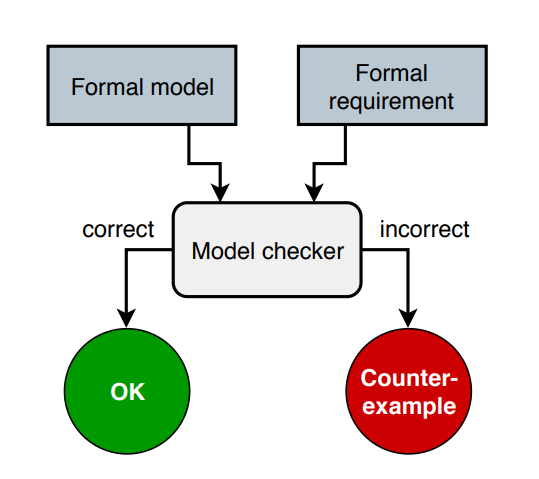
\includegraphics[width=67mm, keepaspectratio]{figures/model_checking.png}\hspace{1cm}
	\caption{An illustration of model checking.}
	\label{fig:model_checking}
\end{figure}

Formal verification tools require the formal model and a formal requirement as input, and return either an ok state, a counter example, or that it can't decide (see \autoref{fig:model_checking}). The counter example is the most important of all, as with its help, the engineers may have a chance of correcting the model.
